\documentclass[12pt]{report}

%%%%%%%%%%%%%%%%%%%%%%%%%%%%%%%%%%%%%%%%%%%%%%%%%%%%%%%%

%%% General Packages
\usepackage{amsmath, amssymb, amsthm}
\usepackage{titling}
\usepackage{titlesec}
\usepackage{geometry}

\usepackage[hidelinks]{hyperref}


%%% Font and Text Packages
\usepackage{newpxtext}
\usepackage{newpxmath}

\usepackage[dvipsnames]{xcolor}


%%% Graphics, Figure and Listing Packages
\usepackage{graphicx}
\usepackage{float}
\usepackage{calc}
\usepackage{caption}
\usepackage{subcaption}


%%% Listings
\usepackage{listings}
\usepackage{lstfiracode}


%%% Bibliography Packages
\usepackage[style=alphabetic]{biblatex}
\bibliography{references}

%%%%%%%%%%%%%%%%%%%%%%%%%%%%%%%%%%%%%%%%%%%%%%%%%%%%%%%%

%%% Page Formatting Options
\geometry{left = 2.5cm}
\geometry{right = 2.5cm}
\geometry{top = 2.5cm}
\geometry{bottom = 2.5cm}

%%% Section and Chapter Titling Options
\titleformat{\chapter}[block]
  {\normalfont\Large\bfseries}{Chapter \thechapter}{1em}{\Large}
\titlespacing*{\chapter}{0pt}{40pt}{30pt}
\titleformat*{\section}{\large\bfseries}

%%% Hyperlink Formatting Options
\hypersetup{
    colorlinks,
    linkcolor={black},
    citecolor={blue!60!black},
    urlcolor={blue!80!black}
}

%%%%%%%%%%%%%%%%%%%%%%%%%%%%%%%%%%%%%%%%%%%%%%%%%%%%%%%%

%%% Graphics and Figure Options
% Graphics path (necessary for .svg images).
\graphicspath{{graphics/}}
\counterwithout{figure}{chapter}

% Caption setup
\captionsetup{margin=1.5cm}


%%% Listings Options
\definecolor{codegreen}{rgb}{0,0.6,0}
\definecolor{codegray}{rgb}{0.5,0.5,0.5}
\definecolor{codepurple}{rgb}{0.58,0,0.82}
\definecolor{codeback}{rgb}{0.95,0.95,0.92}
\lstset{
	language=Python,
	backgroundcolor=\color{codeback},   
	commentstyle=\color{codegreen},
	keywordstyle=\color{magenta},
	numberstyle=\tiny\color{codegray},
	style=FiraCodeStyle,   % Use predefined FiraCodeStyle
	basicstyle=\ttfamily,   % Use \ttfamily for source code listings
	numbers=left
}

%%%%%%%%%%%%%%%%%%%%%%%%%%%%%%%%%%%%%%%%%%%%%%%%%%%%%%%%

%%% Personal Macros
\newcommand{\N}{\mathbb{N}}
\newcommand{\R}{\mathbb{R}}
\newcommand{\Z}{\mathbb{Z}}
\renewcommand{\S}{\mathbb{S}}
\newcommand{\ip}[2]{\langle #1, #2 \rangle}

%%% Drafting Macros
\newcommand{\notered}[1]{{\color{Red} \textbf{#1}}}
\newcommand{\notegreen}[1]{{\color{Green} \textbf{#1}}}
\newcommand{\noteblue}[1]{{\color{Blue} \textbf{#1}}}

%%% Theorem Options
\newtheorem*{theorem}{Theorem}
\newtheorem*{proposition}{Proposition}

%%%%%%%%%%%%%%%%%%%%%%%%%%%%%%%%%%%%%%%%%%%%%%%%%%%%%%%%

\begin{document}
	
%%% Make titlepage.

% Titlepage Options
\author{Damian Lin}
\title{Virtualising the $d$-invariant}

\cleardoublepage \thispagestyle{empty}
\null \vfil
\begingroup
\LARGE \bfseries \centering
\openup \medskipamount
\thetitle \par \vspace{30pt}
\centering \mdseries \theauthor \par \bigskip
\endgroup
\vfil \vfil \vfil
\begin{center}
	An essay submitted in partial fulfilment of\\
	the requirements for the degree of\\
	Bachelor of Science/Bachelor of Advanced Studies (Honours)
	\vfil\vfil
	{\large Pure Mathematics\\[5pt]
		University of Sydney}\\
	\vskip6mm
	\includegraphics[width=25mm]{graphics/USY_MB1_CMYK_Stacked_Logo}
	\vfil
	\normalsize\today
\end{center}
\vfil
\cleardoublepage

\tableofcontents


\chapter*{Introduction}
\addcontentsline{toc}{chapter}{Introduction}

Introduce, Introduce, Introduce.

In order to keep this text relatively self-contained, we begin in Chapter 2 with the study of knots, for without motivating the bread and butter of knot theory: knot invariants, it is hard to motivate so much of the material we encounter later. This provides some motivation for the rest of this chapter in which we slowly build our way up to a a specific invariant, the $d$-invariant, closely following the work of Greene \cite{lattices-graphs-mutation}. In Chapter 3, we examine virtual knots, a generalisation of knots with a multitude of equivalent formulations that allows knots to have diagrams on a any orientable surface. The aim of this is to extend Greene's $d$-invariant to the virtual setting, and examine what properties it is able to hold on to in this new environment. In particular, we find that we suspect the virtual $d$-invariant is less powerful than another invariant known as the Gordon-Litherland Linking Form, and we examine their relationship in chapter $4$ with the hope in chapter $5$ of finding an example to prove this strengthening. In chapter $6$ we examine an algorithm to compute these invariants, and present a proof that indeed, the virtual $d$-invariant is not as strong as the Gordon-Litherland Linking Form, and therefore not a complete mutation invariant of alternating knots.

\chapter{Knots and their Invariants}

\section{Knots}

We begin with the rich and marvellous study of tangled-up pieces of string; the theory of knots. Despite being a complex and intricate field of study, any child can intuitively grasp the concept of a knot as a closed loop of string sitting in space. To formalise this and remove any pathological examples that are inconsistent with our intuition of our inner child, we define a \textit{knot} to be an injective embedding of the circle into $3$-space, $K: \S^{1} \lhook\joinrel\longrightarrow \R^{3}$. The requirement that the embedding be injective ensures that our string does not intersect itself anywhere, and we know it must be closed as an embedding of $\S^{1}$.

\begin{figure}[hbt]
	\centering
	\hfill
	\begin{subfigure}[b]{0.3 \textwidth}
		\centering
		\def\svgscale{0.2}
		\input{graphics/unknot.pdf_tex}
		\caption{Unknot or Trivial Knot}
	\end{subfigure}
	\hfill
	\begin{subfigure}[b]{0.3 \textwidth}
		\centering
		\def\svgscale{0.2}
		\input{graphics/trefoil.pdf_tex}
		\caption{Trefoil Knot}
	\end{subfigure}
	\hfill
	\begin{subfigure}[b]{0.3 \textwidth}
		\centering
		\def\svgscale{0.2}
		\input{graphics/trefoil.pdf_tex}
		\caption{Trefoil Knot \notered{change}}
	\end{subfigure}
	\caption{Some examples of knots.}
	\hfill \phantom{1}
\end{figure}

The natural question that arises as soon as we see something such as in Fig. \ref{fig:unknot_twisted} is when do we consider two knots to be the `same'? We want two knots to be the same if there is some way to deform one, without breaking the circle or passing it through itself, into the other. Hence we say two knots $K_{1}$ and $K_{2}$ are \textit{equivalent} or equal if there is some homeomorphism of the ambient space $\R^{3}$ that restricts to a homeomorphism of the two knots. We call this notion of equivalence ambient isotopy. Knot theory is the study of knots up to ambient isotopy.

\notegreen{Talk about diagrams, alternating knots, Reidemeister moves and (briefly) invariants. Then talk about mutation a little and give some diagrams.} For the rest of this chapter, we largely follow the work of \cite{lattices-graphs-mutation} to introduce the $d$-invariant, which is an mutation invariant of alternating knots.

\begin{figure}[hbt]
	\centering
	\includegraphics[width=0.25\linewidth]{graphics/unknot_twisted}
	\caption{Also the unknot}
	\label{fig:unknot_twisted}
\end{figure}

\section{The Lattice of Integer Flows and the $d$-invariant}
A \textit{lattice} is a finitely generated abelian group $L$, equipped with an inner product 
\(\ip{\cdot}{\cdot}: L \times L \longrightarrow \R\). We are primarily interested in \textit{integral lattices}, for which the inner product's image is contained within $\Z$, and for the rest of this work we assume that all lattices are integral. An \textit{isomorphism of lattices} is a bijection $\psi: L_{1} \longrightarrow L_{2}$ that preserves the inner product, that is $\ip{x}{y} = \ip{\psi(x)}{\psi(y)}$ for all $x, y \in L$.

Throughout, we let $G = (E, V)$ be a finite, directed, connected graph (in which loops and multiple edges are allowed) with vertex set $V$ and edge set $E$. The boundary map $\partial:  C_{0}(G) \longrightarrow C_{1}(G)$ defines a $|V|\times|E|$ incidence matrix $D : \Z^{E} \longrightarrow \Z^{V}$ with entries given by
\[D_{ij} = \begin{cases}
	+1 & \text{if $e_{i}$ is oriented into $v_{j}$}   \\
	-1 & \text{if $e_{i}$ is oriented out of $v_{j}$} \\
	0  & \text{otherwise.}
\end{cases}\]

The \textit{lattice of integer flows} of $G$ is the group $\Lambda(G) = \ker D$, along with the inner product induced by the Euclidean inner product on $\Z^{E}$. Equivalently, $\Lambda(G)$ is the first homology group of $G$, with inner products taken in $C_{1}(G)$. While the lattice $\Lambda(G)$ may depend on the orientation of the edges in $G$, its isomorphism class does not, as the isomorphism class of the homology group is independent of orientation, and the Euclidean inner product is preserved by sending an edge to its negation, since in the Euclidean inner product, $\ip{e_{i}}{e_{i}} =  \ip{-e_{i}}{-e_{i}} = 1$, and $\ip{e_{i}}{e_{j}} = \ip{-e_{i}}{e_{j}} = 0$.

\notegreen{TODO: Perhaps put an example of a lattice of integer flows?}

A \textit{$2$-isomorphism} between two graphs $G = (E, V)$ and $G' = (E', V')$ is a bijection \({\psi: E \longrightarrow E'}\) that preserves cycles, i.e. $\partial(e_{i} + \cdots + e_{j}) = 0$ if and only if $\partial\left(\psi(e_{i}) + \cdots + \psi(e_{j})\right) = 0$. We call and edge $e$ of a graph $G$ a \textit{bridge} if the removal of $G$ from $e$ disconnects $G$, and we say a graph $G$ is \textit{$2$-edge-connected} if $G$ has no bridges.

It is well established that of $2$-edge-connected graphs, $2$-isomorphism implies isomorphic lattices of integer flows; that is $\Lambda(G)$ is a $2$-isomorphism invariant of $2$-edge-connected graphs \parencite{lattice-of-flows-cuts}. More interestingly, and more recently, due to Su-Wagner \cite[Theorem 1]{lattice-of-flows-regular-matroid} and Caporaso-Viviani \cite[Theorem 3.1.1]{torelli-for-graphs-tropical-curves}, the converse is also true.


\begin{theorem}
For two $2$-edge-connected graphs $G$ and $G'$, $\Lambda(G) \cong \Lambda(G')$ if and only if $G$ and $G'$ are $2$-isomorphic. That is, $\Lambda(G)$ is a complete $2$-isomorphism invariant of $2$-edge-connected graphs.
\end{theorem} $\Lambda(G) \cong \Lambda(G')$ if and only if $G \simeq^{2} G'$, that is, the lattice isomorphism class of $\Lambda(G)$ is a complete $2$-isomorphism invariant of graphs.

Two graphs $G$ and $G'$ are related by a \textit{Whitney flip} if it is possible to find two disjoint graphs $\Gamma_{1}$, with distinguished vertices $u_{1}$ and $v_{1}$ and $\Gamma_{2}$ with distinguished vertices $u_{2}$ and $v_{2}$, such that the identifications $u_{1} = u_{2} = u$ and $v_{1} = v_{2} = v$ form $G$, and the identifications $u_{1} = v_{2} = u'$ and $v_{1} = u_{2} = v'$ form $G'$. An example of graphs related by a Whitney flip is given in Fig. \ref{fig:whitney_flip}.

\begin{figure}[hbt]
	\centering
	\def\svgscale{0.5}
	\input{graphics/whitney_flip.pdf_tex}
	
	\caption{An example of a Whitney flip.}
	\label{fig:whitney_flip}
\end{figure}

It is clear that sequences of Whitney flips only ever transform graphs within their $2$-isomorphism class, as cycles map to cycles. From \cite{2-isomorphic-graphs}, we have the important converse; a Reidermeister-like theorem for $2$-isomorphic graphs.

\begin{theorem}[Whitney's Theorem]
Two graphs $G$ and $G'$ are $2$-isomorphic if-and-only-if there is a sequence of Whitney flips relating $G$ to $G'$.
\end{theorem}

\section{Alternating Knots, Mutation and Flyping}
An alternating knot

\chapter{Virtual Knots}

\chapter{Gordon-Litherland Linking Form}

\chapter{Gauss Codes and Knot Algorithms}


\chapter{Computing Mock Seifert Matrices}

\newpage
\printbibliography[title=References]


\appendix

\chapter{Algorithm}


\end{document}

